\documentclass[11pt, a4paper]{article}
\usepackage[utf8]{inputenc}
\usepackage[left=2.35cm, right=3.35cm, top=3.35cm, bottom=3.0cm]{geometry}
\usepackage{amsmath, amssymb, amsthm}
\usepackage[english]{babel}
\usepackage{graphicx}
\usepackage[font={small,it}]{caption}
\graphicspath{ {figures/} }
\usepackage{url}
\usepackage{appendix}
\usepackage{float}
\usepackage{multirow}
\usepackage[bottom]{footmisc}
\usepackage{titling}
\usepackage{subcaption}
\usepackage{wrapfig}
\usepackage[numbered,autolinebreaks,useliterate]{mcode}
\begin{document}

\begin{titlepage}
  \begin{center}
    
    
\includegraphics[scale=1.5]{figures/kuleuven_logo.pdf}~\\[4.5cm]
    \textsc{\Large Master of bioinformatics}\\[0.5cm]

    % Title
    \rule{\linewidth}{0.3mm}\\[0.4cm]
    {\huge \bfseries Support Vector Machines} \\[0.4cm]
    {\large Assignment 2: Function estimation and Time-series prediction} \\[0.4cm]
    \rule{\linewidth}{0.3mm}\\[0.4cm]
    {\large Spring 2016} \\[1.0cm]
    
    % Author and supervisor
    \begin{minipage}{0.4\textwidth}
      \begin{flushleft} \large
        \emph{Author:}\\
	Cedric \textsc{Lood}
      \end{flushleft}
    \end{minipage}
%     %\hfill
    \begin{minipage}{0.4\textwidth}
      \begin{flushright} \large
        \emph{Supervisors:} \\
        Dr. Carlos \textsc{Alaiz}\\
        Dr. Emanuele \textsc{Frandi}\\
        Prof. Johan \textsc{Suykens}\\
        \hfill \newline 
      \end{flushright}
    \end{minipage}
    
    \vfill

    
\includegraphics[scale=0.15]{figures/KUL.jpg}~\\[0.5cm]

    % Bottom of the page
    {\large \today}
    
  \end{center}
\end{titlepage}

\tableofcontents
\newpage

\section*{Context}

The analysis presented in this report was produced for the class of
``Support Vector Machines: methods and applications'' (Spring 2016) at
KU Leuven. The goal is to display understanding of the techniques and
of their practical use. This second report focuses on function
estimation and time series prediction using SVM, and Least-Squares SVM
(LS-SVM). The implementation was done using the MatLab software
(v2015a) and the libraries for LS-SVM developed at KU Leuven
\footnote{http://www.esat.kuleuven.be/sista/lssvmlab/}.

\section{Support Vector Machine for regression}

\subsection{Datasets}
I experimented with 3 noiseless datasets of 20 observations for this
section, based on the true underlying function shown in figure
\ref{fig:regress_datasets}. I used the ``load dataset'' functionality
of the \emph{uiregress} function to load them and perform the regress:

\begin{lstlisting}
X = (linspace(-5, 5, 20))'; Y = (2.*X + 1)';
save('lin.mat');

X = (linspace(-5,5,20))'; Y = (X.^3 + X.^2 - 1)';
save('poly.mat');

X = (linspace(-pi,pi,20))'; Y = (exp(-X.^2).*sin(10.*X))';
save('sinc.mat');
\end{lstlisting}

\begin{figure}[H]
    \centering
    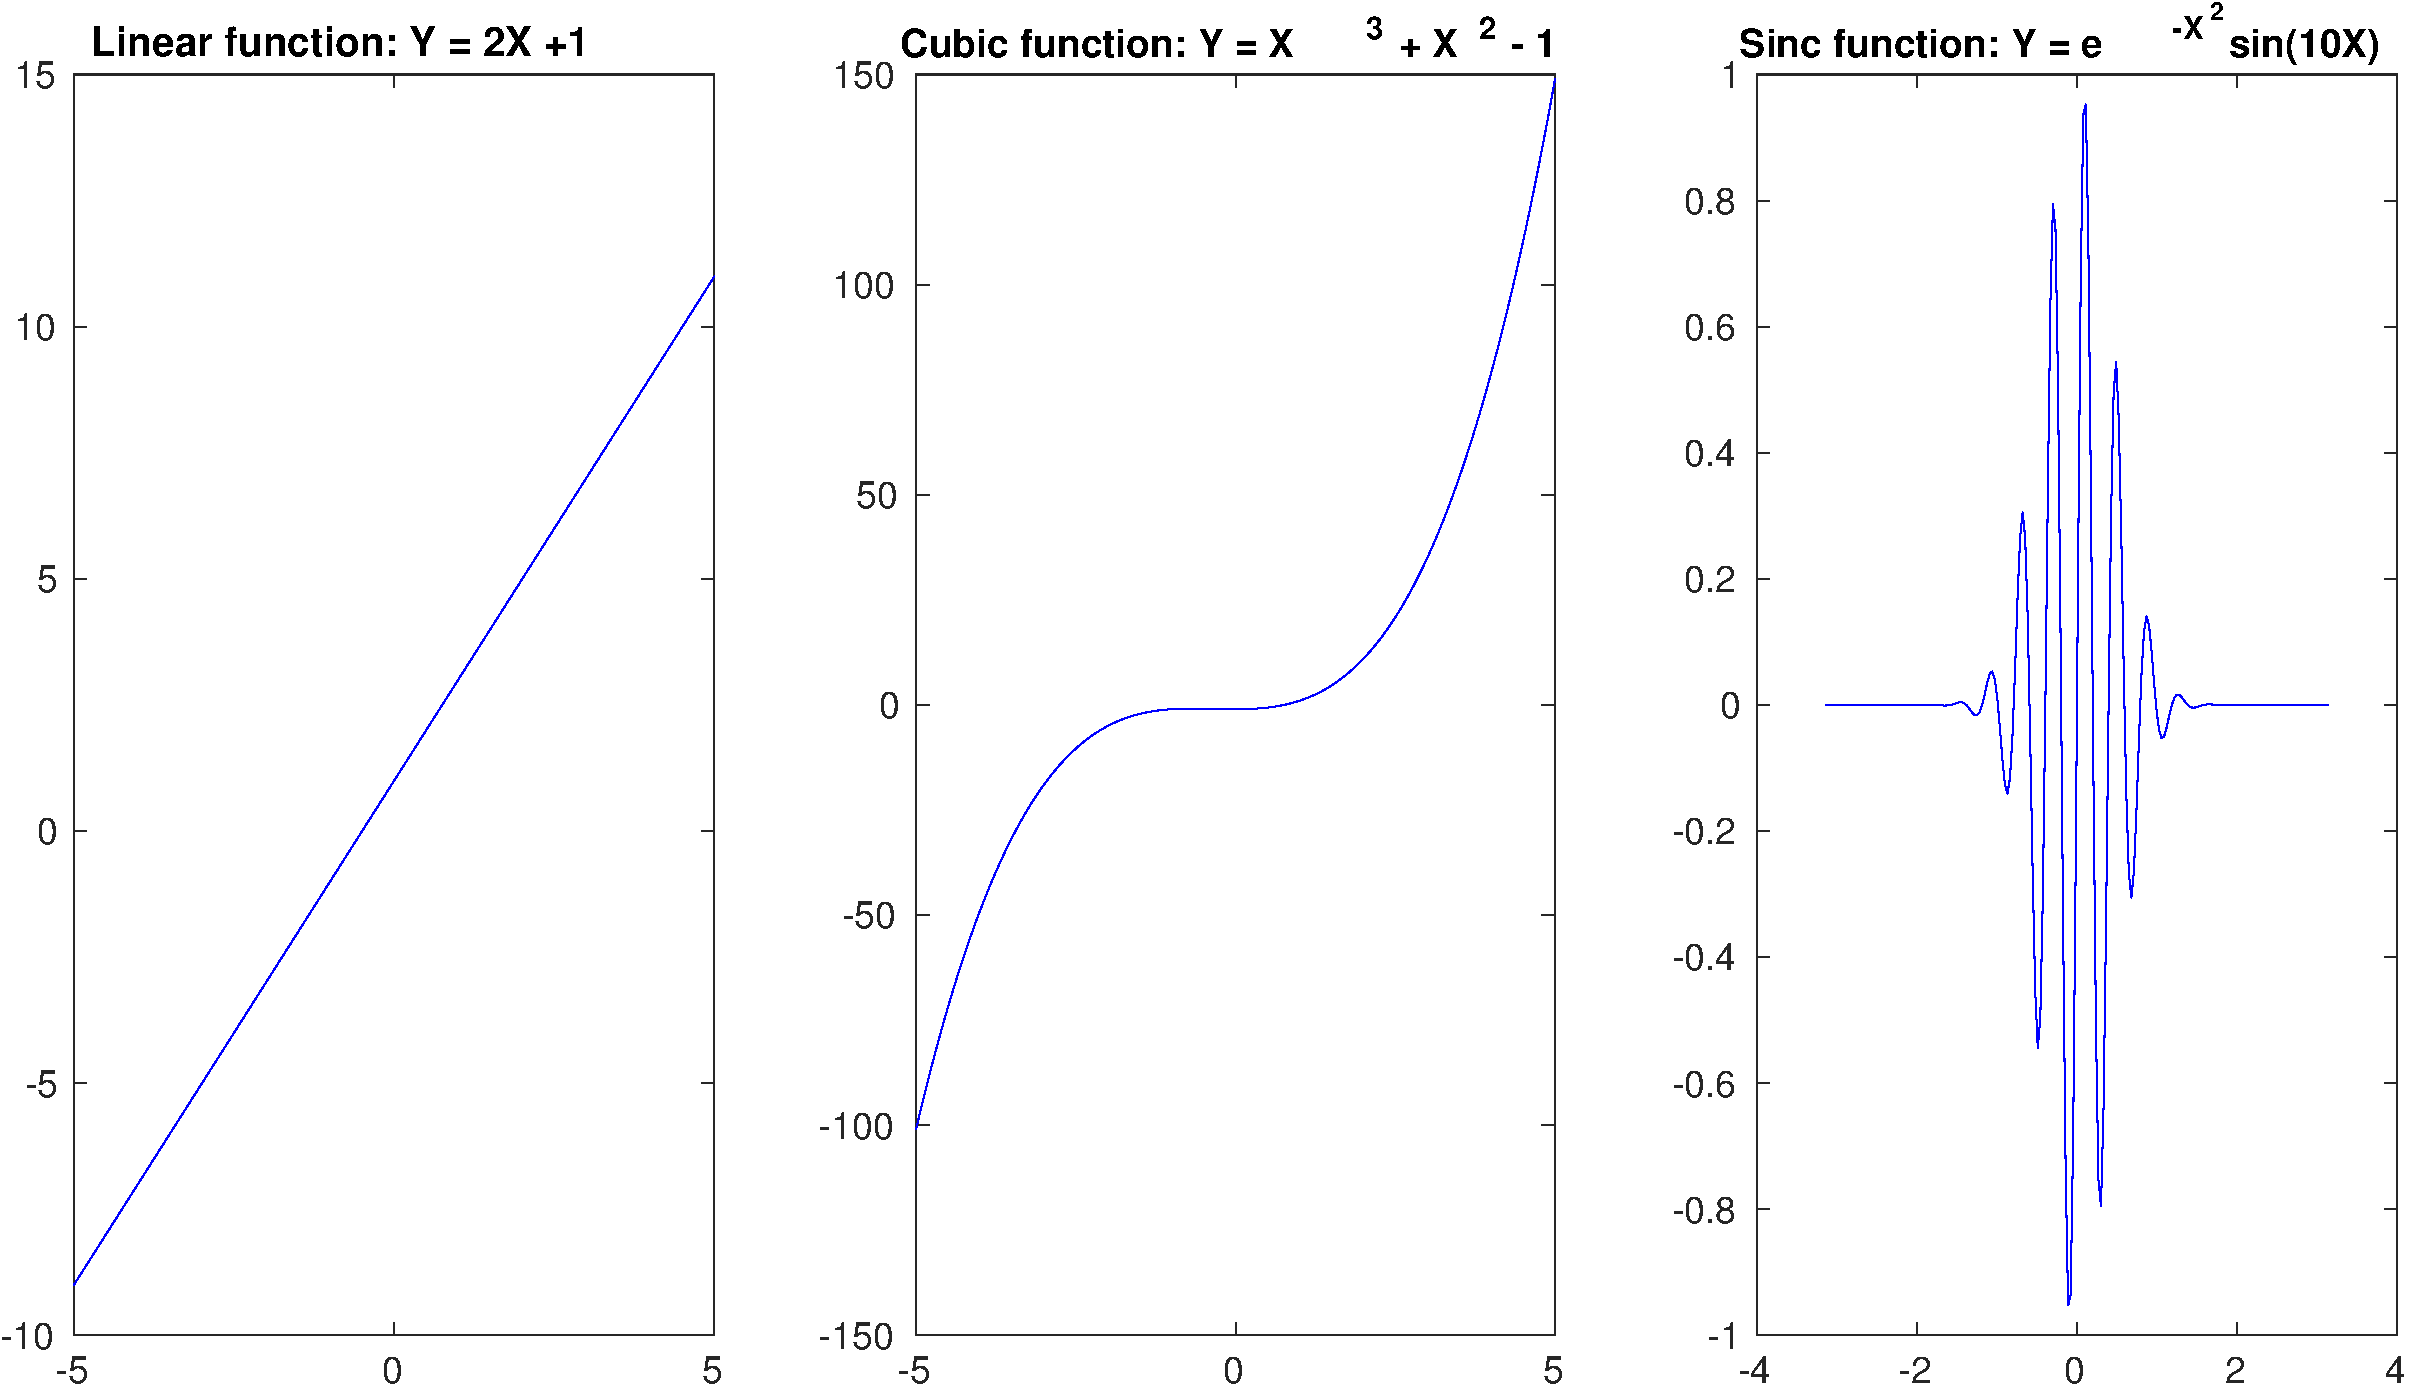
\includegraphics[scale=.30]{datasets.pdf}
    \caption{Functions to regress}
    \label{fig:regress_datasets}
\end{figure}

\subsection{Analysis}

Here we investigate the effect of fixing the amount of different
settings on the function estimation:

\begin{itemize}
\item $\epsilon$ or \emph{e} controls the loss function
\item $\sigma$ controls the bandwidth of the RBF kernel
\item the polynomial degree (1 means linear kernel)
\item $\gamma$ or \emph{bound} controls the amount of regularization
  (hence the smoothness of the decision boundary)
\end{itemize}

For the linear and cubic generated dataset, I got good results with
polynomial kernel of degree 1 and 3 respectively. In general, the RBF
kernel worked well on all the dataset.

I did an extensive survey of the parameters for the first linear
dataset. On that particular set, the linear kernel seem to have
performed the best. Even for extremely low $\epsilon$ (eg
$\epsilon=0.005$), the number of support vectors needed to describe
the classifier is equal to two. Another obvious advantage of that
kernel was that no wiggle artefact appeared, in contrast with the
other more flexible kernels. Note that this performance was achievable
using the RBF kernel too, using a very large $\sigma$ (as large values
of that parameter tend to make decision boundaries linear).

\begin{table}[H]
  \centering
  \begin{tabular}{l|r|r|r|r|r|r|r|r|r|r|}
    \cline{2-11}
    & \multicolumn{5}{l|}{e-value (Bound set to Inf)}                                                                                                 & \multicolumn{5}{l|}{Bound (e-value set to 0.1)}                                                                                           \\ \cline{2-11} 
    & \multicolumn{1}{l|}{0.005} & \multicolumn{1}{l|}{0.01} & \multicolumn{1}{l|}{0.05} & \multicolumn{1}{l|}{0.1} & \multicolumn{1}{l|}{0.5} & \multicolumn{1}{l|}{0.01} & \multicolumn{1}{l|}{0.1} & \multicolumn{1}{l|}{1} & \multicolumn{1}{l|}{10} & \multicolumn{1}{l|}{100} \\ \hline
    \multicolumn{1}{|l|}{Poly 1}             & 2                          & 2                         & 2                         & 2                        & 2                        & 20 **                     & 20 **                    & 13                     & 2                       & 100                      \\ \hline
    \multicolumn{1}{|l|}{Poly 2}             & 3                          & 6                         & 6                         & 6                        & 3                        & 20 **                     & 20 **                    & 8                      & 3                       & 3                        \\ \hline
    \multicolumn{1}{|l|}{Poly 3}             & 7                          & 7                         & 4                         & 4                        & 2 *                      & 20 **                     & 20 **                    & 15 *                   & 4 *                     & 4 *                      \\ \hline
    \multicolumn{1}{|l|}{Poly 4}             & 5                          & 5                         & 5                         & 5                        & 4 *                      & 20 **                     & 20 **                    & 14 *                   & 5 *                     & 5 *                      \\ \hline
    \multicolumn{1}{|l|}{RBF $\sigma^2=1$}   & 16                         & 7                         & 7                         & 4                        & 4 *                      & 20 **                     & 20 **                    & 20 **                  & 15 **                   & 4                        \\ \hline
    \multicolumn{1}{|l|}{RBF $\sigma^2=0.5$} & 10                         & 9                         & 9                         & 7                        & 5 *                      & 20 **                     & 20 **                    & 20 **                  & 10 **                   & 7 *                      \\ \hline
  \end{tabular}
  \caption{Number of support vectors required for different kernels and parameters (*: wiggle artefact visible, **: function estimation completely off)}
  \label{table:dataset_lin}
\end{table}

A general remark concerning the regularization applied via the bound
parameter, is that if too little of it is applied, the regression
performs poorly on my artificial datasets. Given that it controls how
error is allowed in the model, this makes sense. The same remark goes
for the e-value, which controls the loss function. If this value is
small, the model doesn't allow for a large margin.

% \begin{figure}[H]
%     \centering
%     \includegraphics[scale=.40]{two_gaussians.pdf}
%     %\caption{Two gaussians classification}
%     \label{fig:two_gaussians}
% \end{figure}

\section{Sum of Cosines}

I started by investigating the regression of the function with a given
$\sigma^2$ value of 0.1, as illustrated by the following code:

\begin{lstlisting}
gam_list = [1000, 100, 10, 1];
sig2_list = [0.1, 0.1, 0.1, 0.1];
figure('Color',[1 1 1]);

for i = 1:4
    gam = gam_list(i); sig2 = sig2_list(i);
    [alpha, b] = trainlssvm({Xtrain, Ytrain, 'f', gam, sig2, 'RBF_kernel'});
    YtestEst = simlssvm({Xtrain, Ytrain, 'f', gam, sig2, 'RBF_kernel'},{alpha, b}, Xtest);
    subplot(2,2,i);
    plot(XX, YY, 'k-'); hold on; 
    plot(Xtest, Ytest, '.'); hold on; 
    plot(Xtest, YtestEst, 'r+');
    legend('true', 'Ytest', 'YtestEst');
end
\end{lstlisting}

The results are visually reported on figure \ref{fig:sumcos1}

\begin{figure}[H]
    \centering
    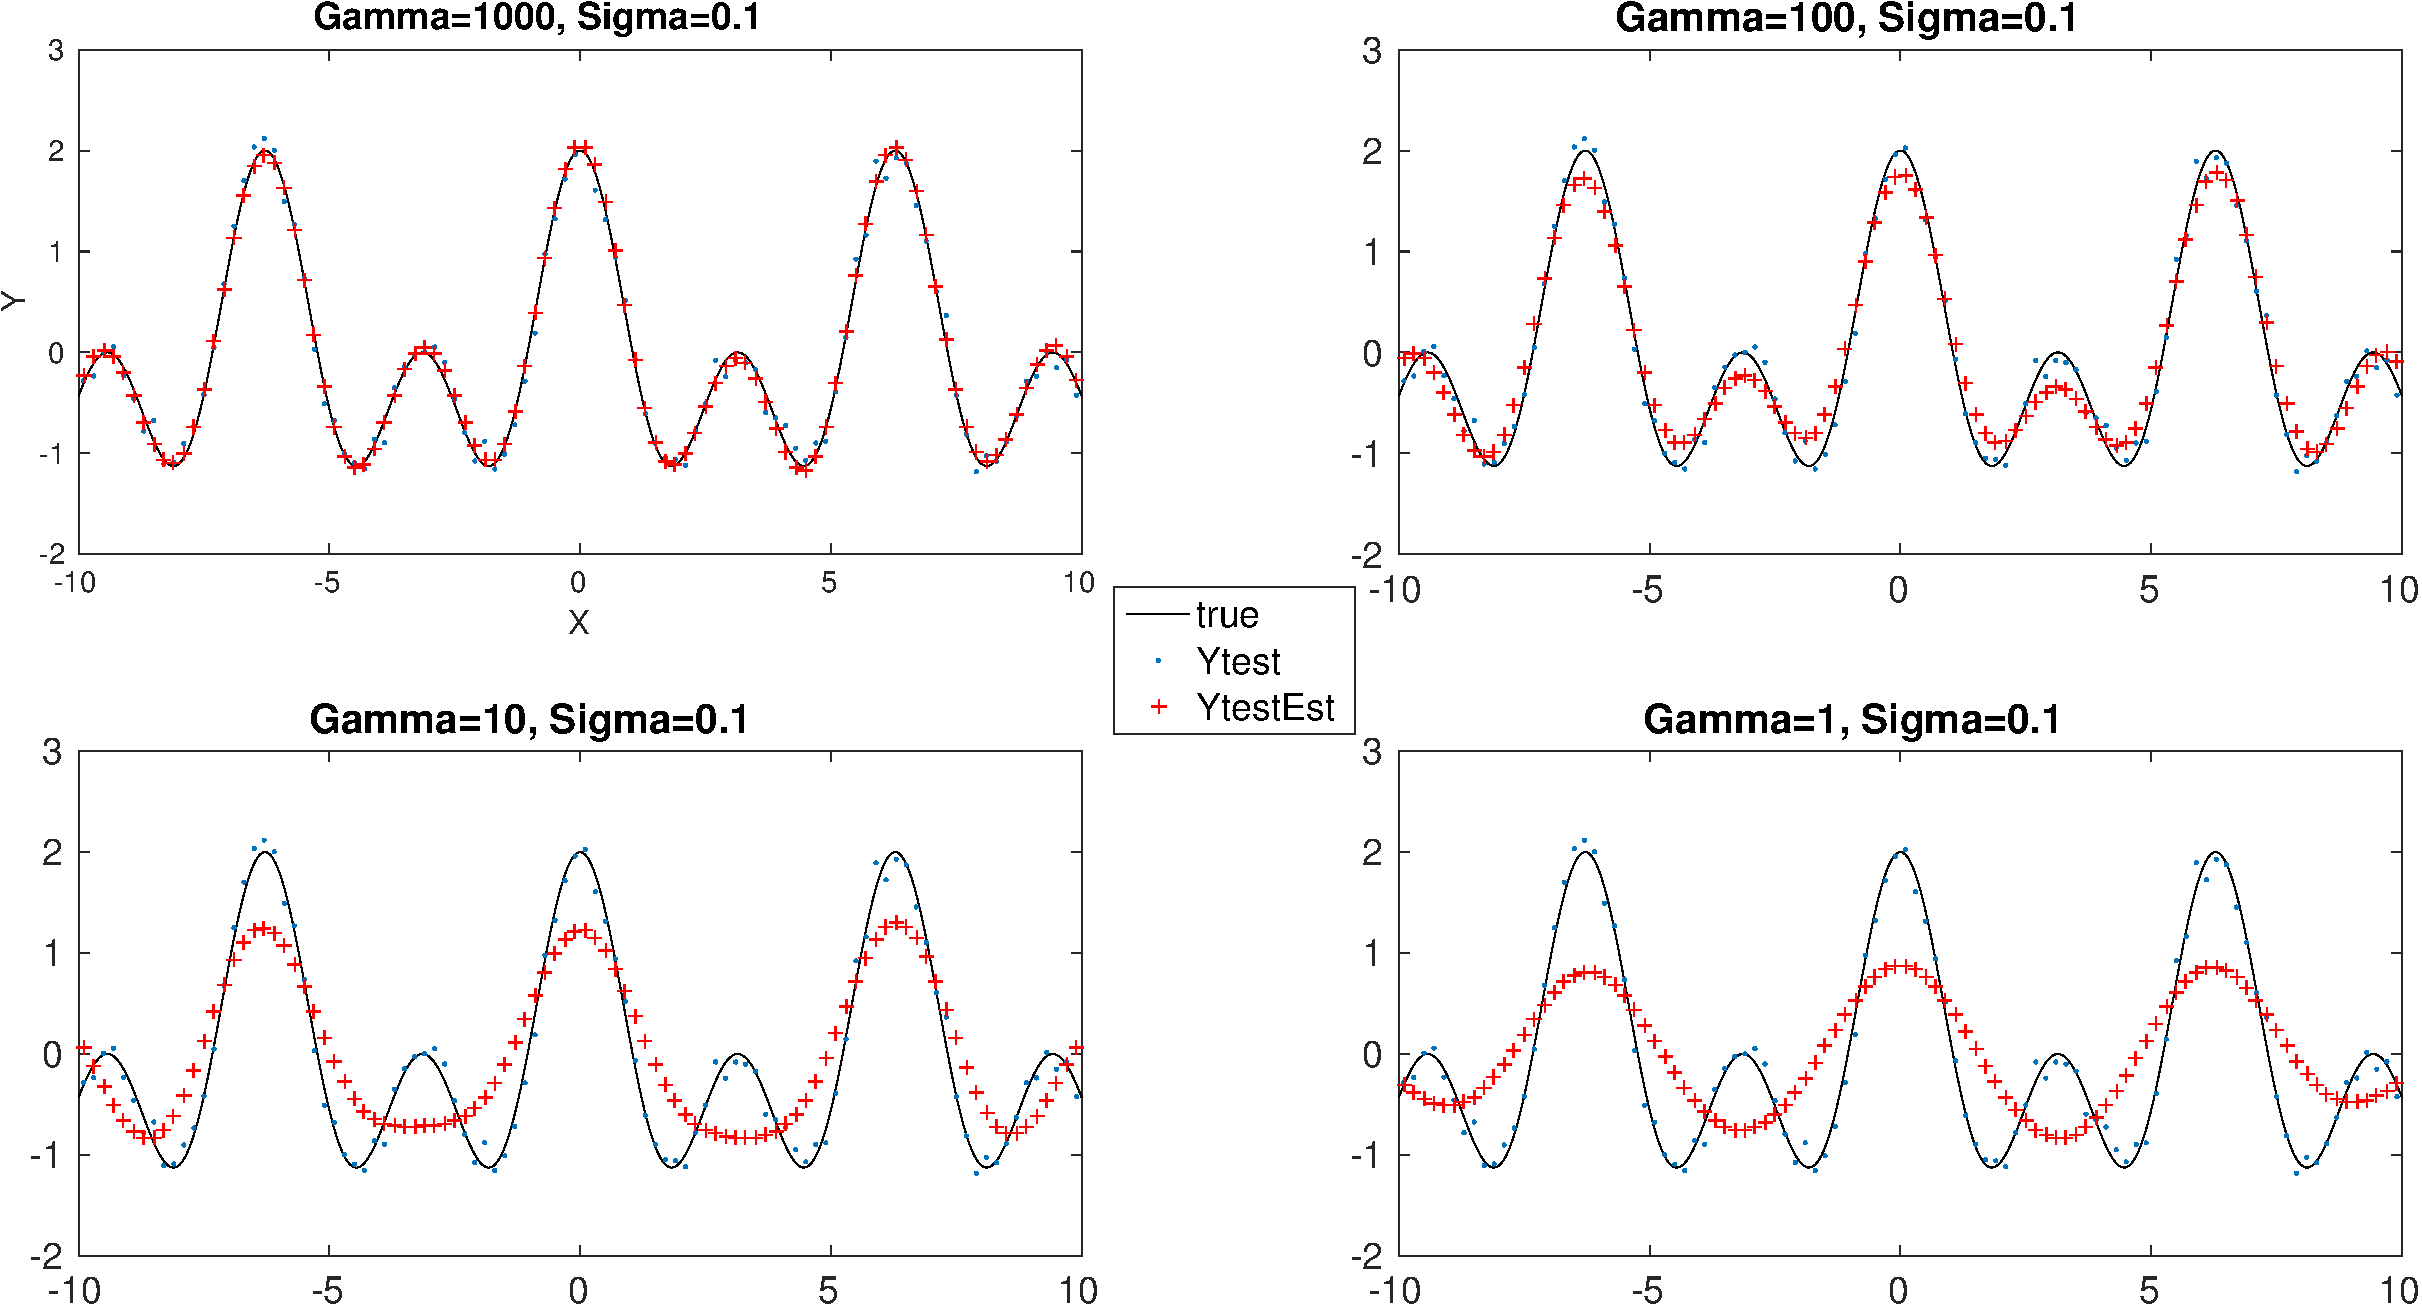
\includegraphics[scale=.40]{sumcos1.pdf}
    \caption{Function estimation for various values of $\gamma$ (fixed
      $\sigma^2$)}
    \label{fig:sumcos1}
\end{figure}

I then investigated the function estimation for a fixed value of
$\gamma$ using similar code. The visual results can be seen on figure
\ref{fig:sumcos2}

\begin{figure}[H]
    \centering
    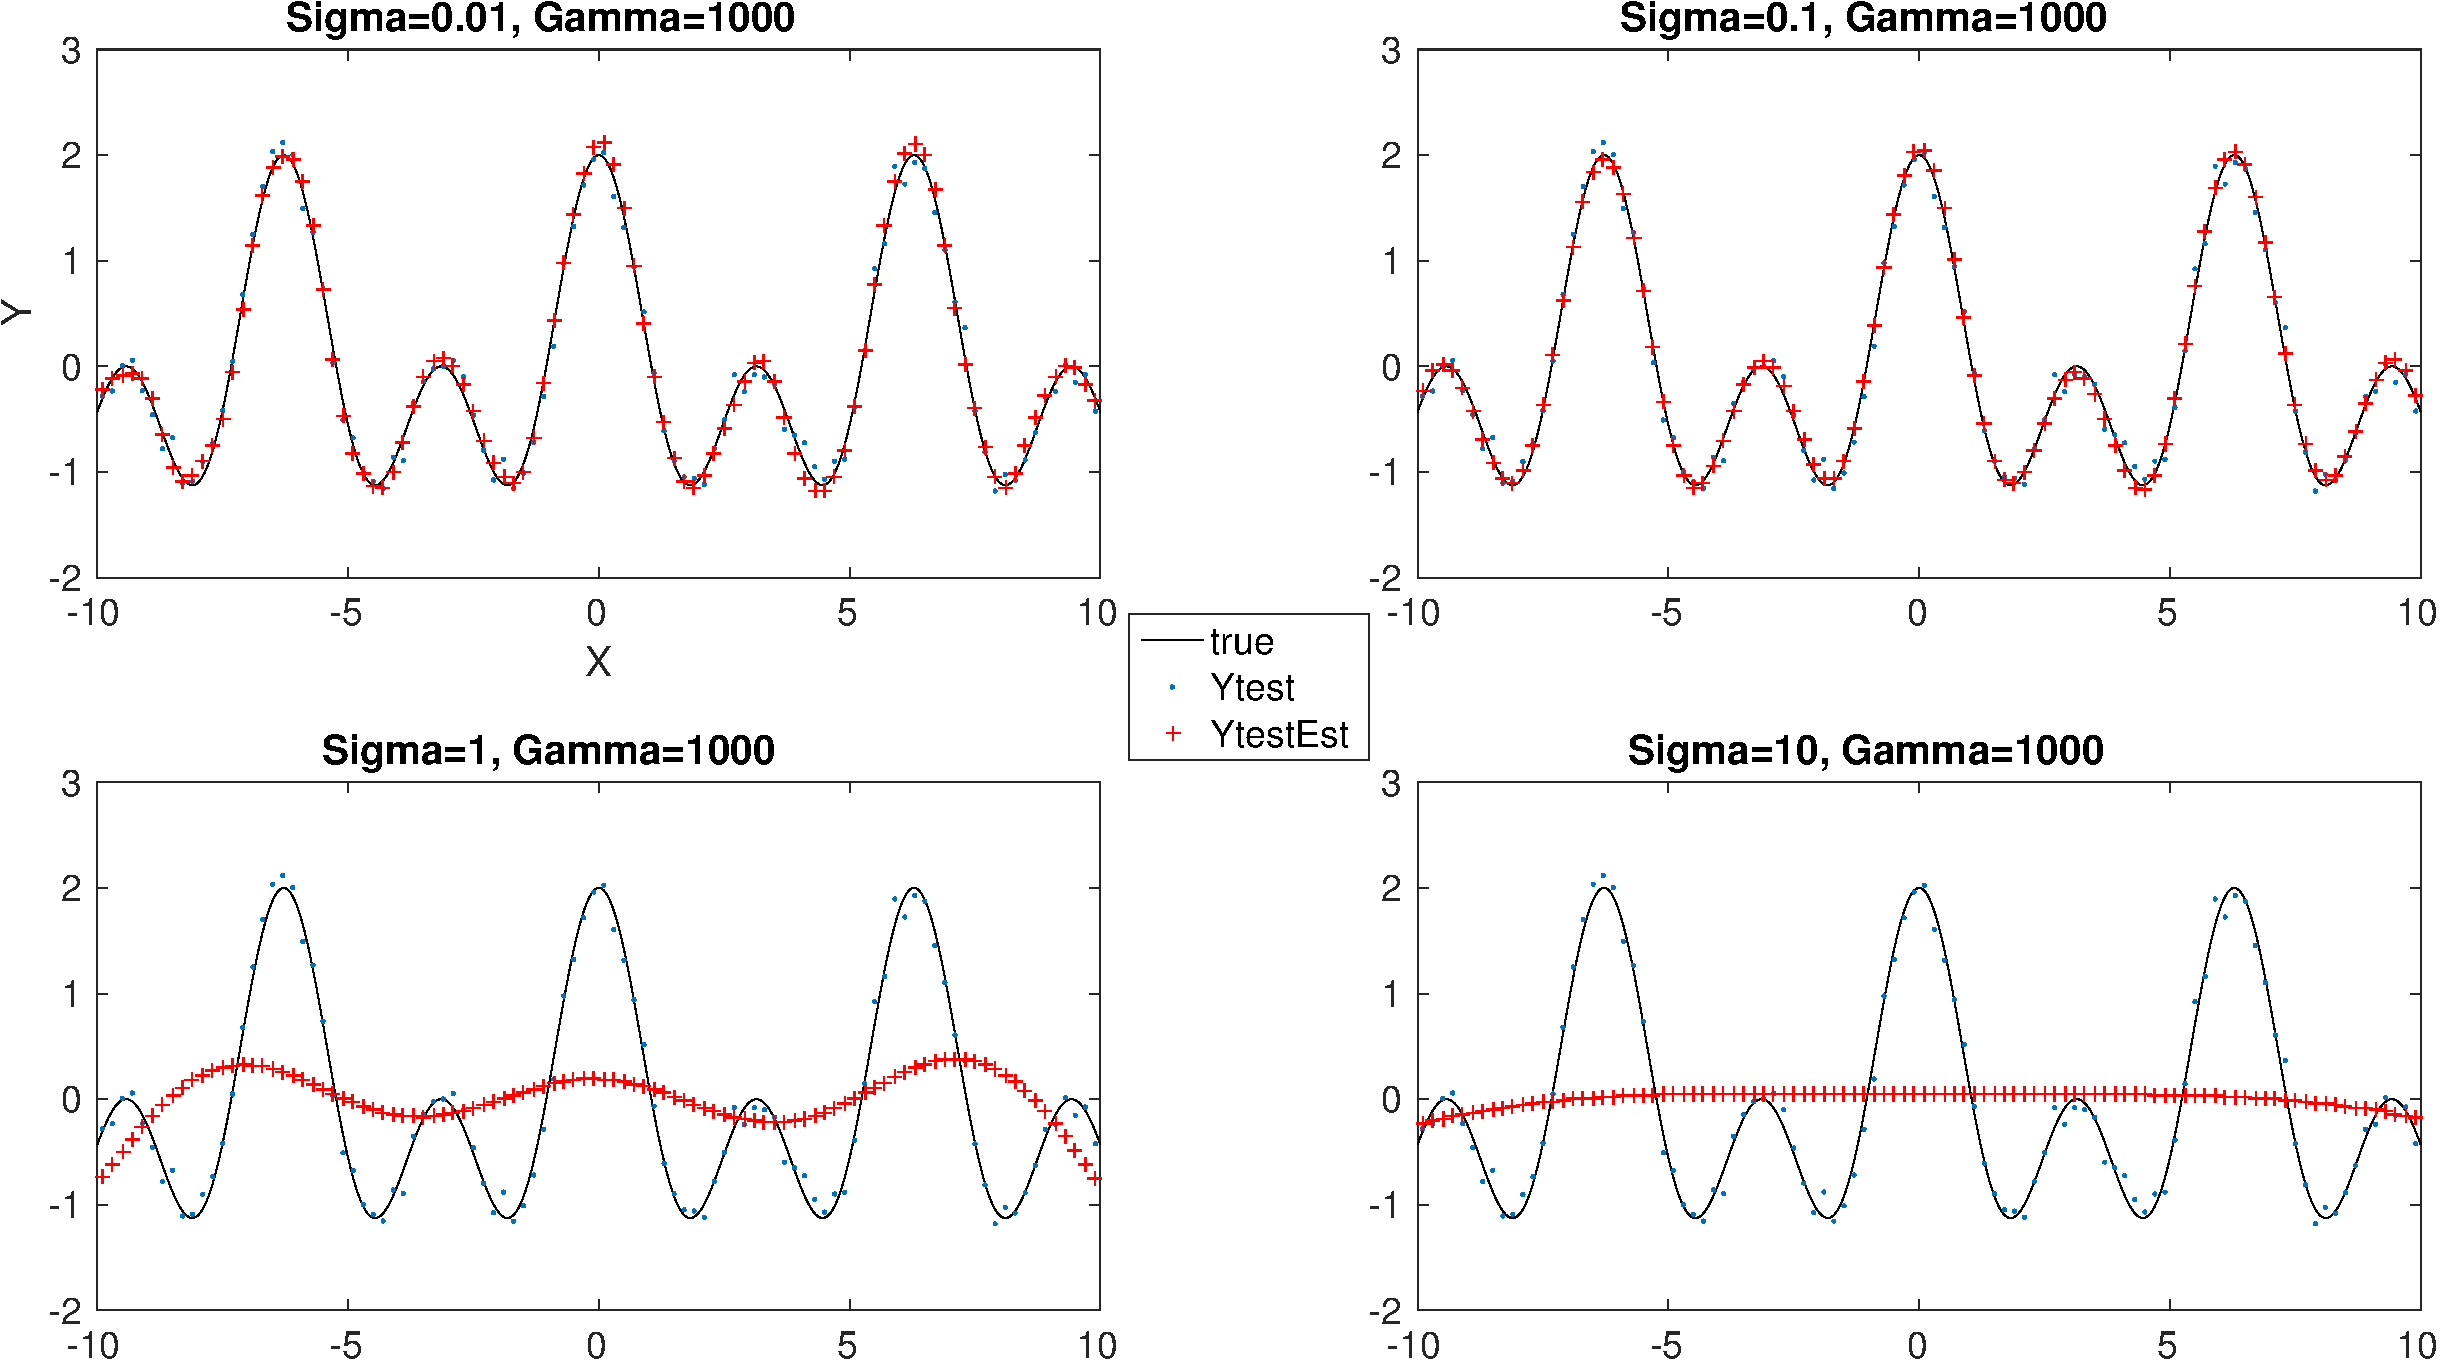
\includegraphics[scale=.40]{sumcos2.pdf}
    \caption{Function estimation for various values of $\sigma^2$ (fixed
      $\gamma$)}
    \label{fig:sumcos2}
\end{figure}

One of the question from this exercise is to determine whether there
is an optimal pair of parameters that would reach the best
estimation. Although the SVM formulation is convex, and thus has a
single solution, when we start exploring hyperparameter space, the
problem is no more convex. 

I thought that there would not be a single pair, and decided to verify
this by computing and visualizing the error surface consisting of
systematic evaluation between the estimated Y for a given pair of
$\sigma^2$ and $\gamma$ and the true Y (known in our case given that
we are working with a synthetic dataset.) Here is the code I used for
this part:

\begin{lstlisting}
gam_list = logspace(-2,2,100); sig2_list = logspace(-2,1,100);
err_matrix = zeros(100,100); i = 1; j = 1;
true_ys = cos(Xtest) + cos(2.*Xtest);

for sig2=sig2_list,
    j = 1;
    for gam=gam_list,
        [alpha, b] = trainlssvm({Xtrain, Ytrain, 'f', gam, sig2, 'RBF_kernel'});
        YtestEst = simlssvm({Xtrain, Ytrain, 'f', gam, sig2, 'RBF_kernel'},{alpha, b}, Xtest);
        err_matrix(i, j) = sum((YtestEst - true_ys).^2);
        j = j + 1;
    end
    i = i + 1;
end

figure('Color',[1,1,1]);
h = surf(gam_list, sig2_list, err_matrix);
set(get(h,'Parent'),'XScale','log');
set(get(h,'Parent'),'YScale','log');
\end{lstlisting}

The result of the parameter space exploration can be seen on figure
\ref{fig:sumcos_surf}. One can recognize that there is indeed no
single best pair of parameters to obtain. In general a large gamma
will reap better results in lowering the error for this synthetic
dataset. For larger $\gamma$, the value of $\sigma^2$ can be larger.

\begin{figure}[H]
    \centering
    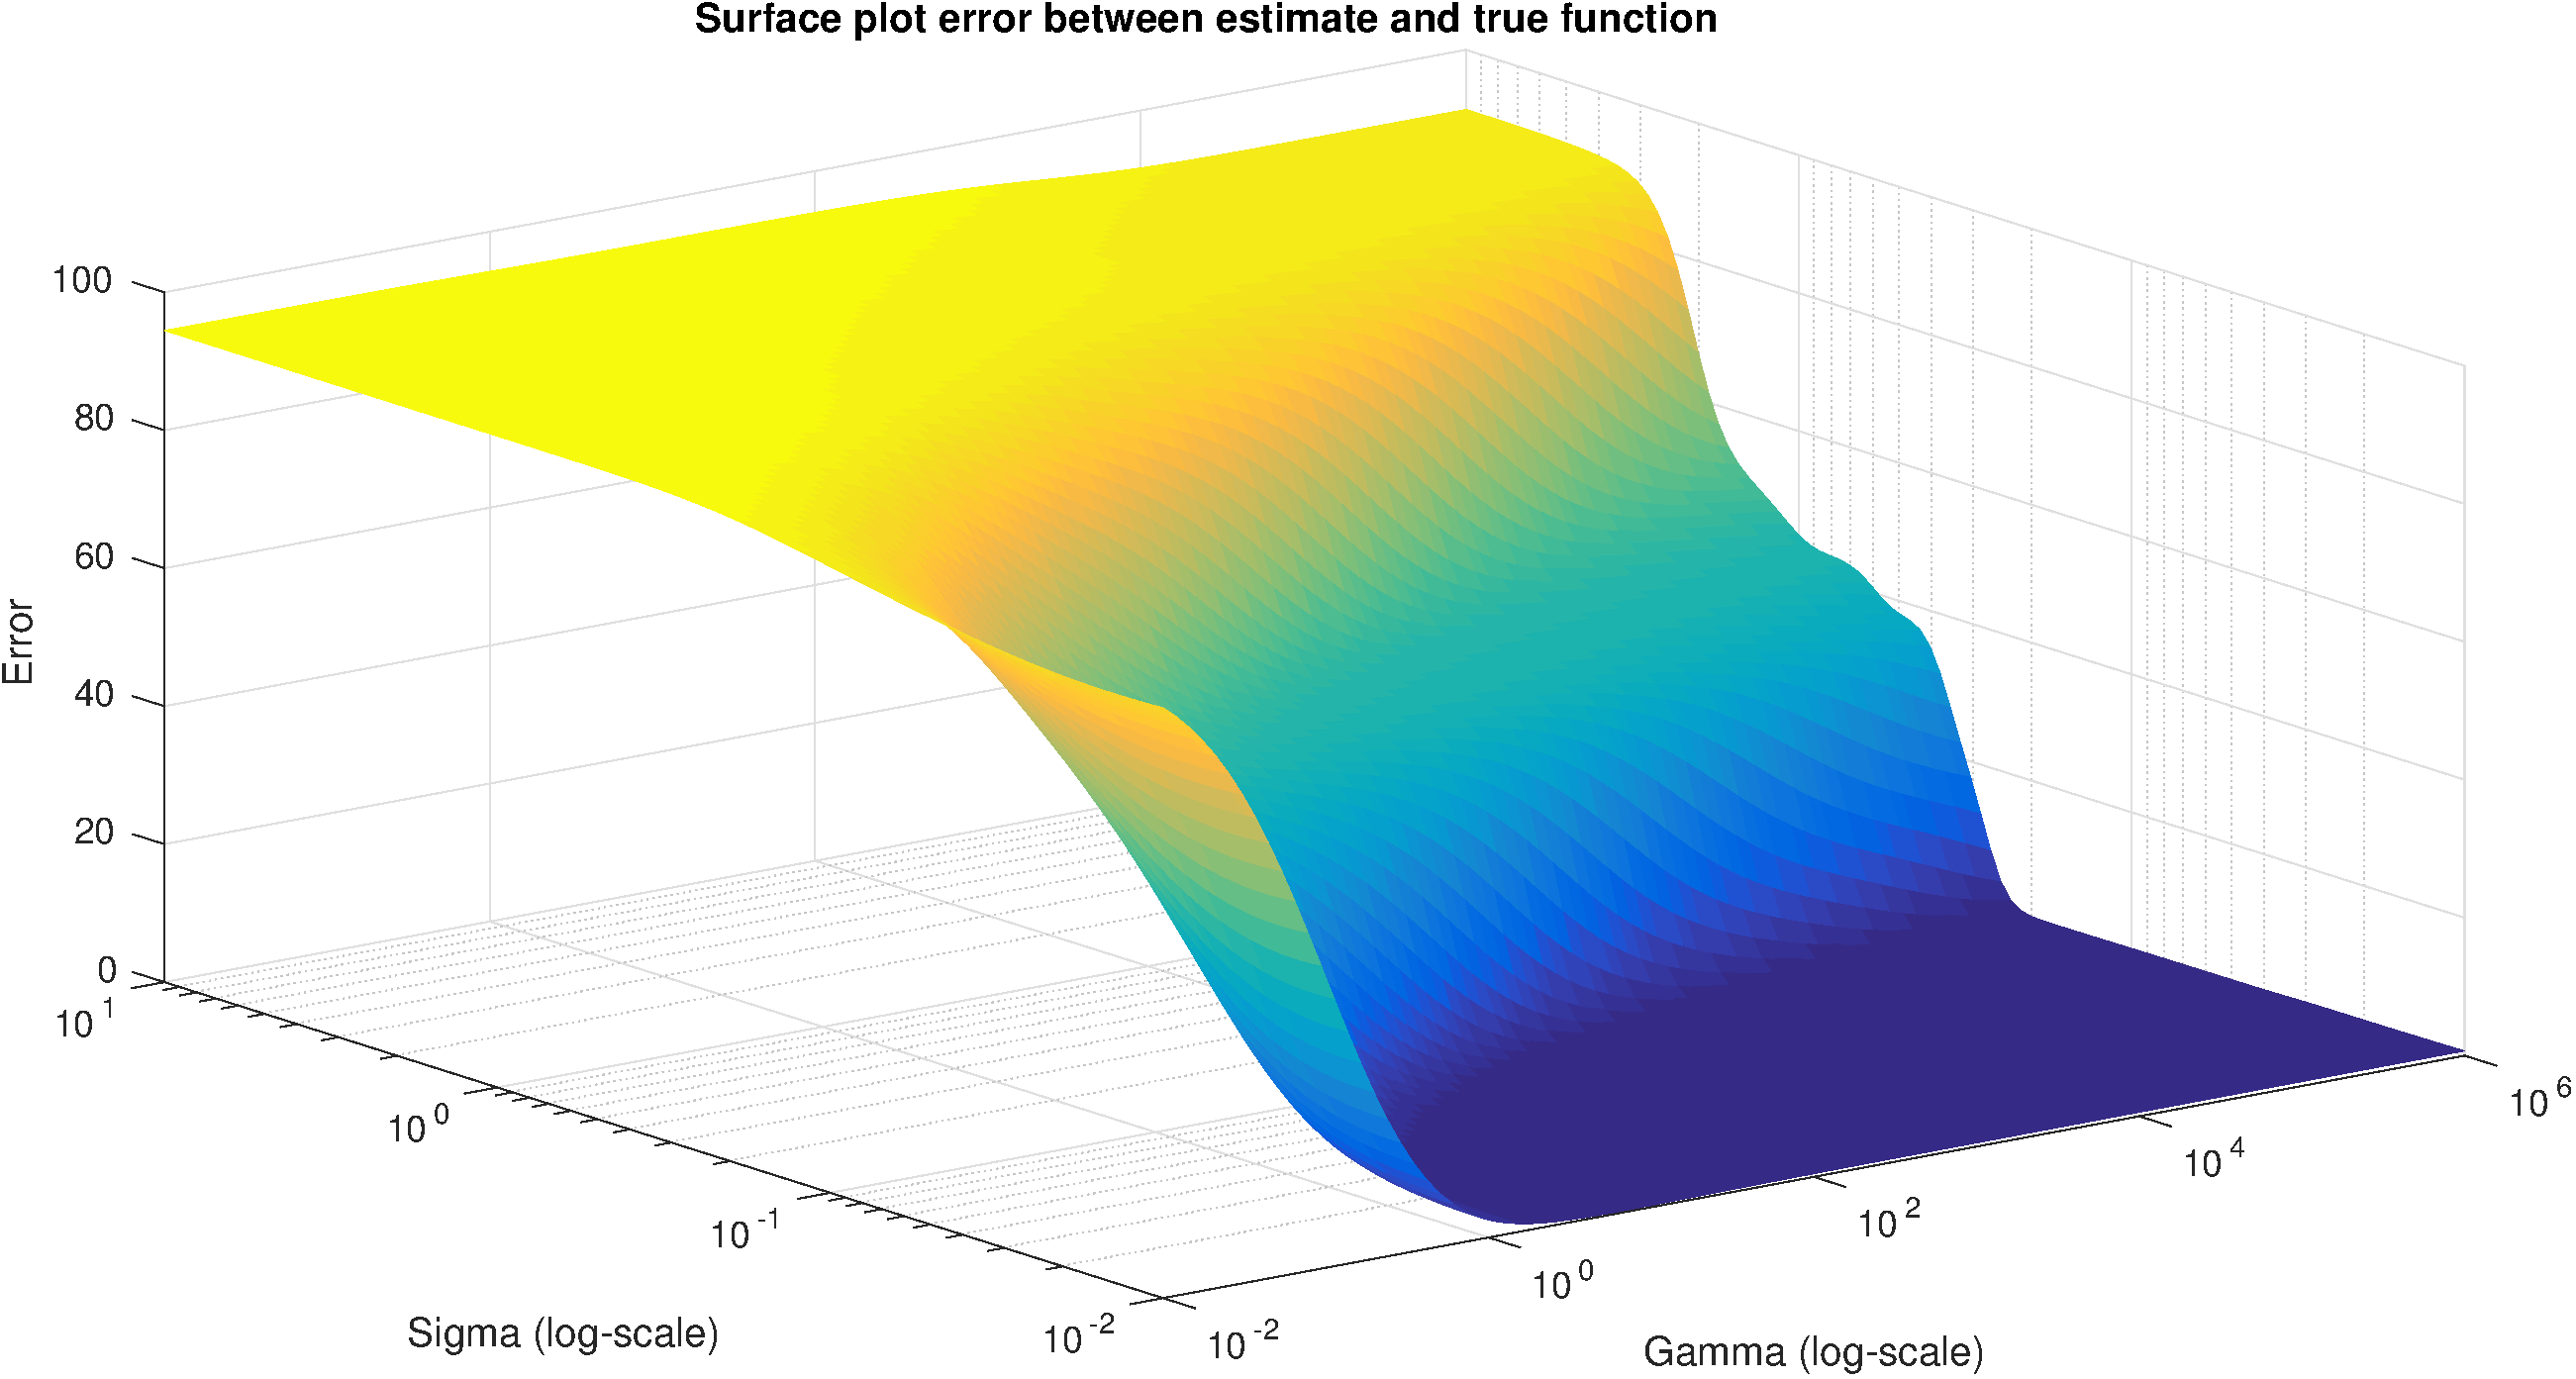
\includegraphics[scale=.40]{sumcos_surf.pdf}
    \caption{Exploration of parameter space effect on the function estimation}
    \label{fig:sumcos_surf}
\end{figure}

\section{Hyper-parameter Tuning}

In order to tune the parameters, I used a combination of the 2 global
optimisation techniques available (coupled-simulated annealing and
randomized directional search) with the 2 techniques to select the
values of the hyperparameters (simplex and gridsearch). I could not
see any difference in the result of the function estimation. All the
values returned were systematically in the area of low test error
discovered in the previous section.

\begin{figure}[H]
    \centering
    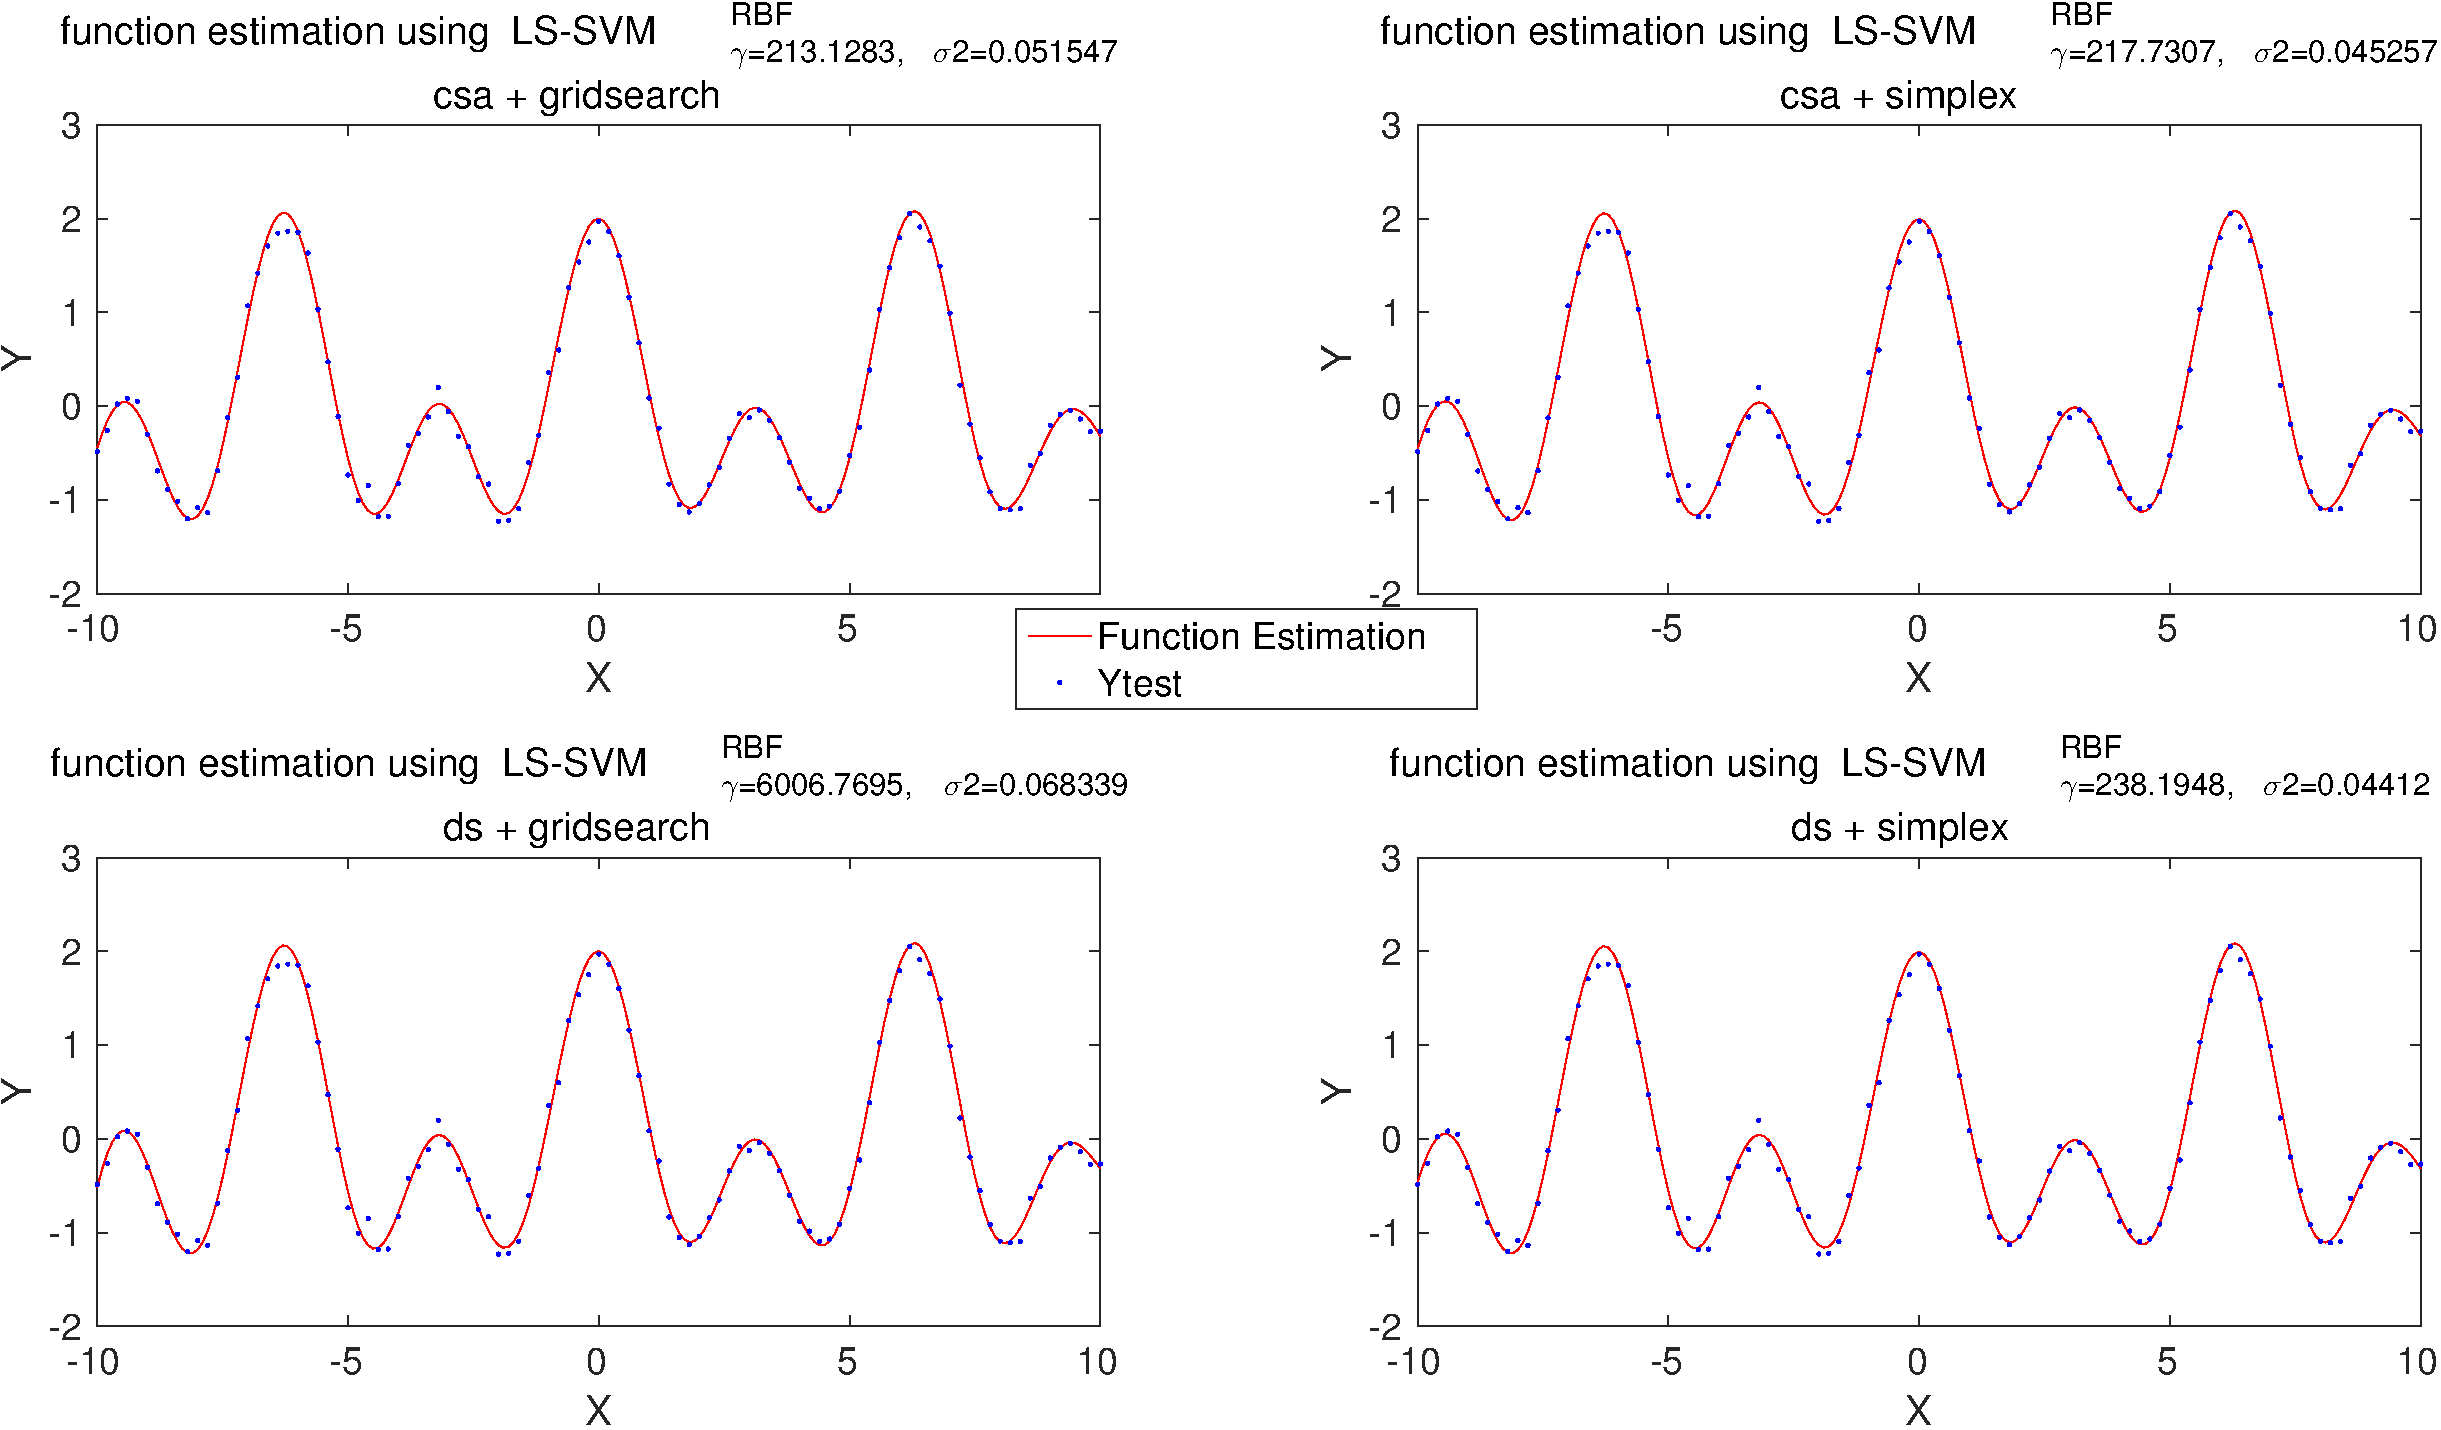
\includegraphics[scale=.40]{hyperparam_tuning.pdf}
    \caption{Parameter tuning with heuristics}
    \label{fig:hyperparam_tuning}
\end{figure}

The speed of execution can be estimated using the tic/toc commands in
matlab. The results in execution time in seconds are reported in table
\ref{tab:computing_param}. It would seem on this small experiment,
that the simplex is faster at moving in the search space of $\gamma$
and $\sigma^2$ than gridsearch. The global optimisation algorithm
coupled simulated annealing (csa) converges to a minimum faster than
the alternative randomized directed search (ds) algorithm.

\begin{table}[H]
  \centering
  \begin{tabular}{l|l|l|l|l|l|l|}
    \cline{2-7}
    & run 1 & run 2 & run 3 & run 4 & run 5 & avg  \\ \hline
    \multicolumn{1}{|l|}{csa + simplex}    & 0.59  & 0.68  & 0.66  & 0.66  & 0.61  & 0.64 \\ \hline
    \multicolumn{1}{|l|}{csa + gridsearch} & 1.01  & 0.92  & 0.95  & 0.92  & 0.91  & 0.94 \\ \hline
    \multicolumn{1}{|l|}{ds + simplex}     & 0.96  & 0.72  & 0.64  & 0.79  & 0.60  & 0.74 \\ \hline
    \multicolumn{1}{|l|}{ds + gridsearch}  & 1.06  & 1.11  & 1.29  & 1.07  & 1.08  & 1.12 \\ \hline
  \end{tabular}
  \caption{Computing time (seconds)}
  \label{tab:computing_param}
\end{table}

% \begin{figure}[H]
%     \centering
%     \begin{subfigure}{.5\textwidth}
%       \centering
%       \includegraphics[width=0.9\linewidth]{1-2-1-kernel7.png}
%       \caption{Support vectors reduce dataset}
%       \label{fig:ker7reduced}
%     \end{subfigure}%
%     \begin{subfigure}{.5\textwidth}
%       \centering
%       \includegraphics[width=0.9\linewidth]{1-2-1-kernel7spiral.png}
%       \caption{No compression}
%       \label{fig:ker7spiral}
%     \end{subfigure}
%     \caption{Support vectors}
%     \label{fig:ker7}
% \end{figure}

\section{Application of the Bayesian framework}

In this section, we investigate the use of the bayes rule for the
tuning and analysis of function approximation (with a quick incursion
in the classification task). The dataset is the same as in the
previous section (sum of cosines).


\section{Robust regression}

\section{Applications}

\subsection{Time-series Prediction}

\subsection{Santa Fe Laser Dataset}

\bibliographystyle{ieeetr} \bibliography{bib-db}
\end{document}
